\documentclass[12pt,letterpaper]{report}
% https://graduate.asu.edu/sites/default/files/asu-graduate-college-format-manual.pdf

% for glossaries and key terms - this file (in the folder) provides its own package to keep things tidy. 
\usepackage{dissglossary}

\usepackage{natbib}
\usepackage{geometry}
\usepackage{fancyhdr}
\usepackage{afterpage}

% this is where the pictures are stored
\usepackage{graphicx}
\graphicspath{ {./images/} } 

\usepackage{amsmath,amssymb,amsbsy}
\usepackage{dcolumn,array}
\usepackage{tocloft} % http://mirrors.ibiblio.org/CTAN/macros/latex/contrib/tocloft/tocloft.pdf

% the styleguide file for ASU specifically.
\usepackage{asudis}


		
\begin{document}
%-----------------------front matter
\pagenumbering{roman}
\title{My Very Good Title\\ \ \\ Very good Subtitle here too.}
\author{Nikki Lane Stevens}
\degreeName{Doctor of Philosophy}
\defensemonth{April}
\gradmonth{May}
\gradyear{2021}
\chair{My first co-chair, Co-Chair \\ My second co-chair, Co-Chair \\ Member Name \\ Member Name \\ Member Name}		
\maketitle
\doublespace
\begin{abstract}string that can uniquely identify it. Primary keys are essential for linking data spread across database tables,
and for looking up and retrieving data from specific records. Yet for an identifier that seems so straightforward
and uncontroversial, we find myriad ways that this unassuming bit of infrastructure has an outsized influence
in human services work. Through case studies of the organizational networks of two nonprofit human services
organizations, we find that different stakeholders use variants of identifiers to support work practices that are
far more complex and social than the linking of tables or the lookup of data. Yet we also find that the low-level
technical properties of the primary key are often coercive, forcing end-users to work on the infrastructure’s
terms—influencing the nature and order of the work, creating new forms of work, and influencing the tenor
of the relationships among stakeholders\end{abstract}
% dedication
\dedicationpage{
  for everyone!
}
% acknowledgements
\acknowledgementpage{
  Thank everyone!

Thank so many people it justifies its own file!
 }
%{Enter your acknowledgement text here}
\tableofcontents
% This puts the word "Page" right justified above everything else.
\addtocontents{toc}{~\hfill Page\par}
% Asking LaTeX for a new page here guarantees that the LOF is on a separate page
% after the TOC ends.
\newpage
% Making the LOT and LOF "parts" rather than chapters gets them indented at
% level -1 according to the chart: top of page 4 of the document at
% ftp://tug.ctan.org/pub/tex-archive/macros/latex/contrib/tocloft/tocloft.pdf

% This gets the headers for the LOT right on the first page.  Subsequent pages
% are handled by the fancyhdr code in the asudis.sty file.

%% for the list of tables, if you need it.
\addcontentsline{toc}{part}{LIST OF TABLES}
\listoftables
\addtocontents{lot}{Table~\hfill Page \par}
\newpage

%% for the list of tables, if you need it. 
\addcontentsline{toc}{part}{LIST OF FIGURES}
\listoffigures
\addtocontents{lof}{Figure~\hfill Page \par}
\newpage

%% for the list of symbols, if you need it
\addcontentsline{toc}{part}{LIST OF SYMBOLS}
\clearpage
\symbolspage{}

%% for the preface, if you have one.
\addcontentsline{toc}{part}{PREFACE}
\clearpage
\addcontentsline{toc}{part}{GLOSSARY AND TERMS}
\clearpage
\addtocontents{toc}{CHAPTER \par}					

%% for the glossary too


% the glossary page needs to be down here too.
\glossarypage{}
\newpage

% the preface content needs to be down here I think? 
\prefacepage{
  this is test preface content.
}


\clearpage
% this line adds the Chapter heading so that the chapters can then exist and get numbered here. 


% This gets the headers for the LOF right on the first page.  Subsequent pages
% are handled by the fancyhdr code in the asudis.sty file.


%-----------------------body
\doublespace
\pagenumbering{arabic}
\chapter{INTRODUCTION - INVITING SURVEILLANCE}
\section{Gallileo's Middle: Finger}
\section{Sorting Things In}

\section{How does software engineering work?}

\subsection{The software development lifecycle}
\cite{noble1979} wrote a lot about the commercialization of engineering, and some early engineering trainings.  

\cite[p.~25]{noble2016a} did a different very good job.  She's also very good. 

I'm not sure if I need to autocite this.\footnote{this is a footnote test, just making sure the style works okay}  But if I wanted to autocite one of my own pieces \cite{stevens2018} that would be pretty tight. And pretty soon I'll have even more.  
Lorem ipsum dolor amet tattooed af keffiyeh biodiesel synth, edison bulb tumblr XOXO hashtag fashion axe readymade gentrify pork belly tousled pug. Pok pok live-edge health goth whatever ennui messenger bag. Kickstarter cardigan chambray 90's, keffiyeh cred pinterest distillery vice \acrfull{wbd} semiotics. Activated charcoal direct trade hashtag, sartorial tbh jean shorts wolf franzen man bun chicharrones vinyl.

Celiac jean shorts fingerstache cardigan. Chicharrones woke lyft kale chips artisan, farm-to-table tofu art party small batch keffiyeh pickled. Man bun heirloom green juice literally typewriter copper mug. Actually direct trade gentrify, flexitarian crucifix organic mumblecore authentic banh mi tattooed occupy whatever fashion axe. Fam edison bulb you probably haven't heard of them authentic iceland trust fund cronut raw denim. Franzen listicle drinking vinegar humblebrag, synth waistcoat af paleo. Pour-over vegan kinfolk leggings VHS authentic.
The \Gls{latex} typesetting markup language is specially suitable 

Cornhole fingerstache retro, butcher freegan chambray ugh. Banh mi palo santo williamsburg messenger bag umami cardigan. Chia fam single-origin coffee viral intelligentsia fanny pack health goth cronut. Leggings XOXO cardigan, sriracha brooklyn poke distillery mumblecore whatever offal master cleanse typewriter plaid freegan. Jianbing keytar snackwave keffiyeh twee poutine man braid.

Fixie thundercats snackwave, pork belly prism scenester vinyl. Heirloom whatever DIY selvage banjo photo booth hell of hashtag godard tote bag sustainable health goth. Palo santo taiyaki photo booth kinfolk cold-pressed, migas pork belly YOLO before they sold out roof party raclette pop-up. Vaporware sustainable pabst tumeric, tumblr pug beard jean shorts.

Butcher ugh portland sartorial flexitarian 8-bit. Chia photo booth small batch, umami af austin literally intelligentsia quinoa pitchfork tilde art party hell of enamel pin. Raclette af gentrify iceland ethical microdosing. Bushwick single-origin coffee taiyaki keffiyeh pug shabby chic. Wayfarers live-edge try-hard, cold-pressed man braid echo park bitters copper mug readymade. 



\chapter{Case Study 1: Such a good chapter, much thinking }
\section{Section1}
% testing the glossary using this entry 
 \Glspl{formula} is a glossary word.  Look how it renders!.
\section{Section2}
\section{Section3}
\section{Pushing the TOC onto 2 pages}
\section{To make sure the headers work}
\chapter{Case Study 2: Another good chapter}
\section{Section1}
\section{Section2}

\begin{figure}[t]
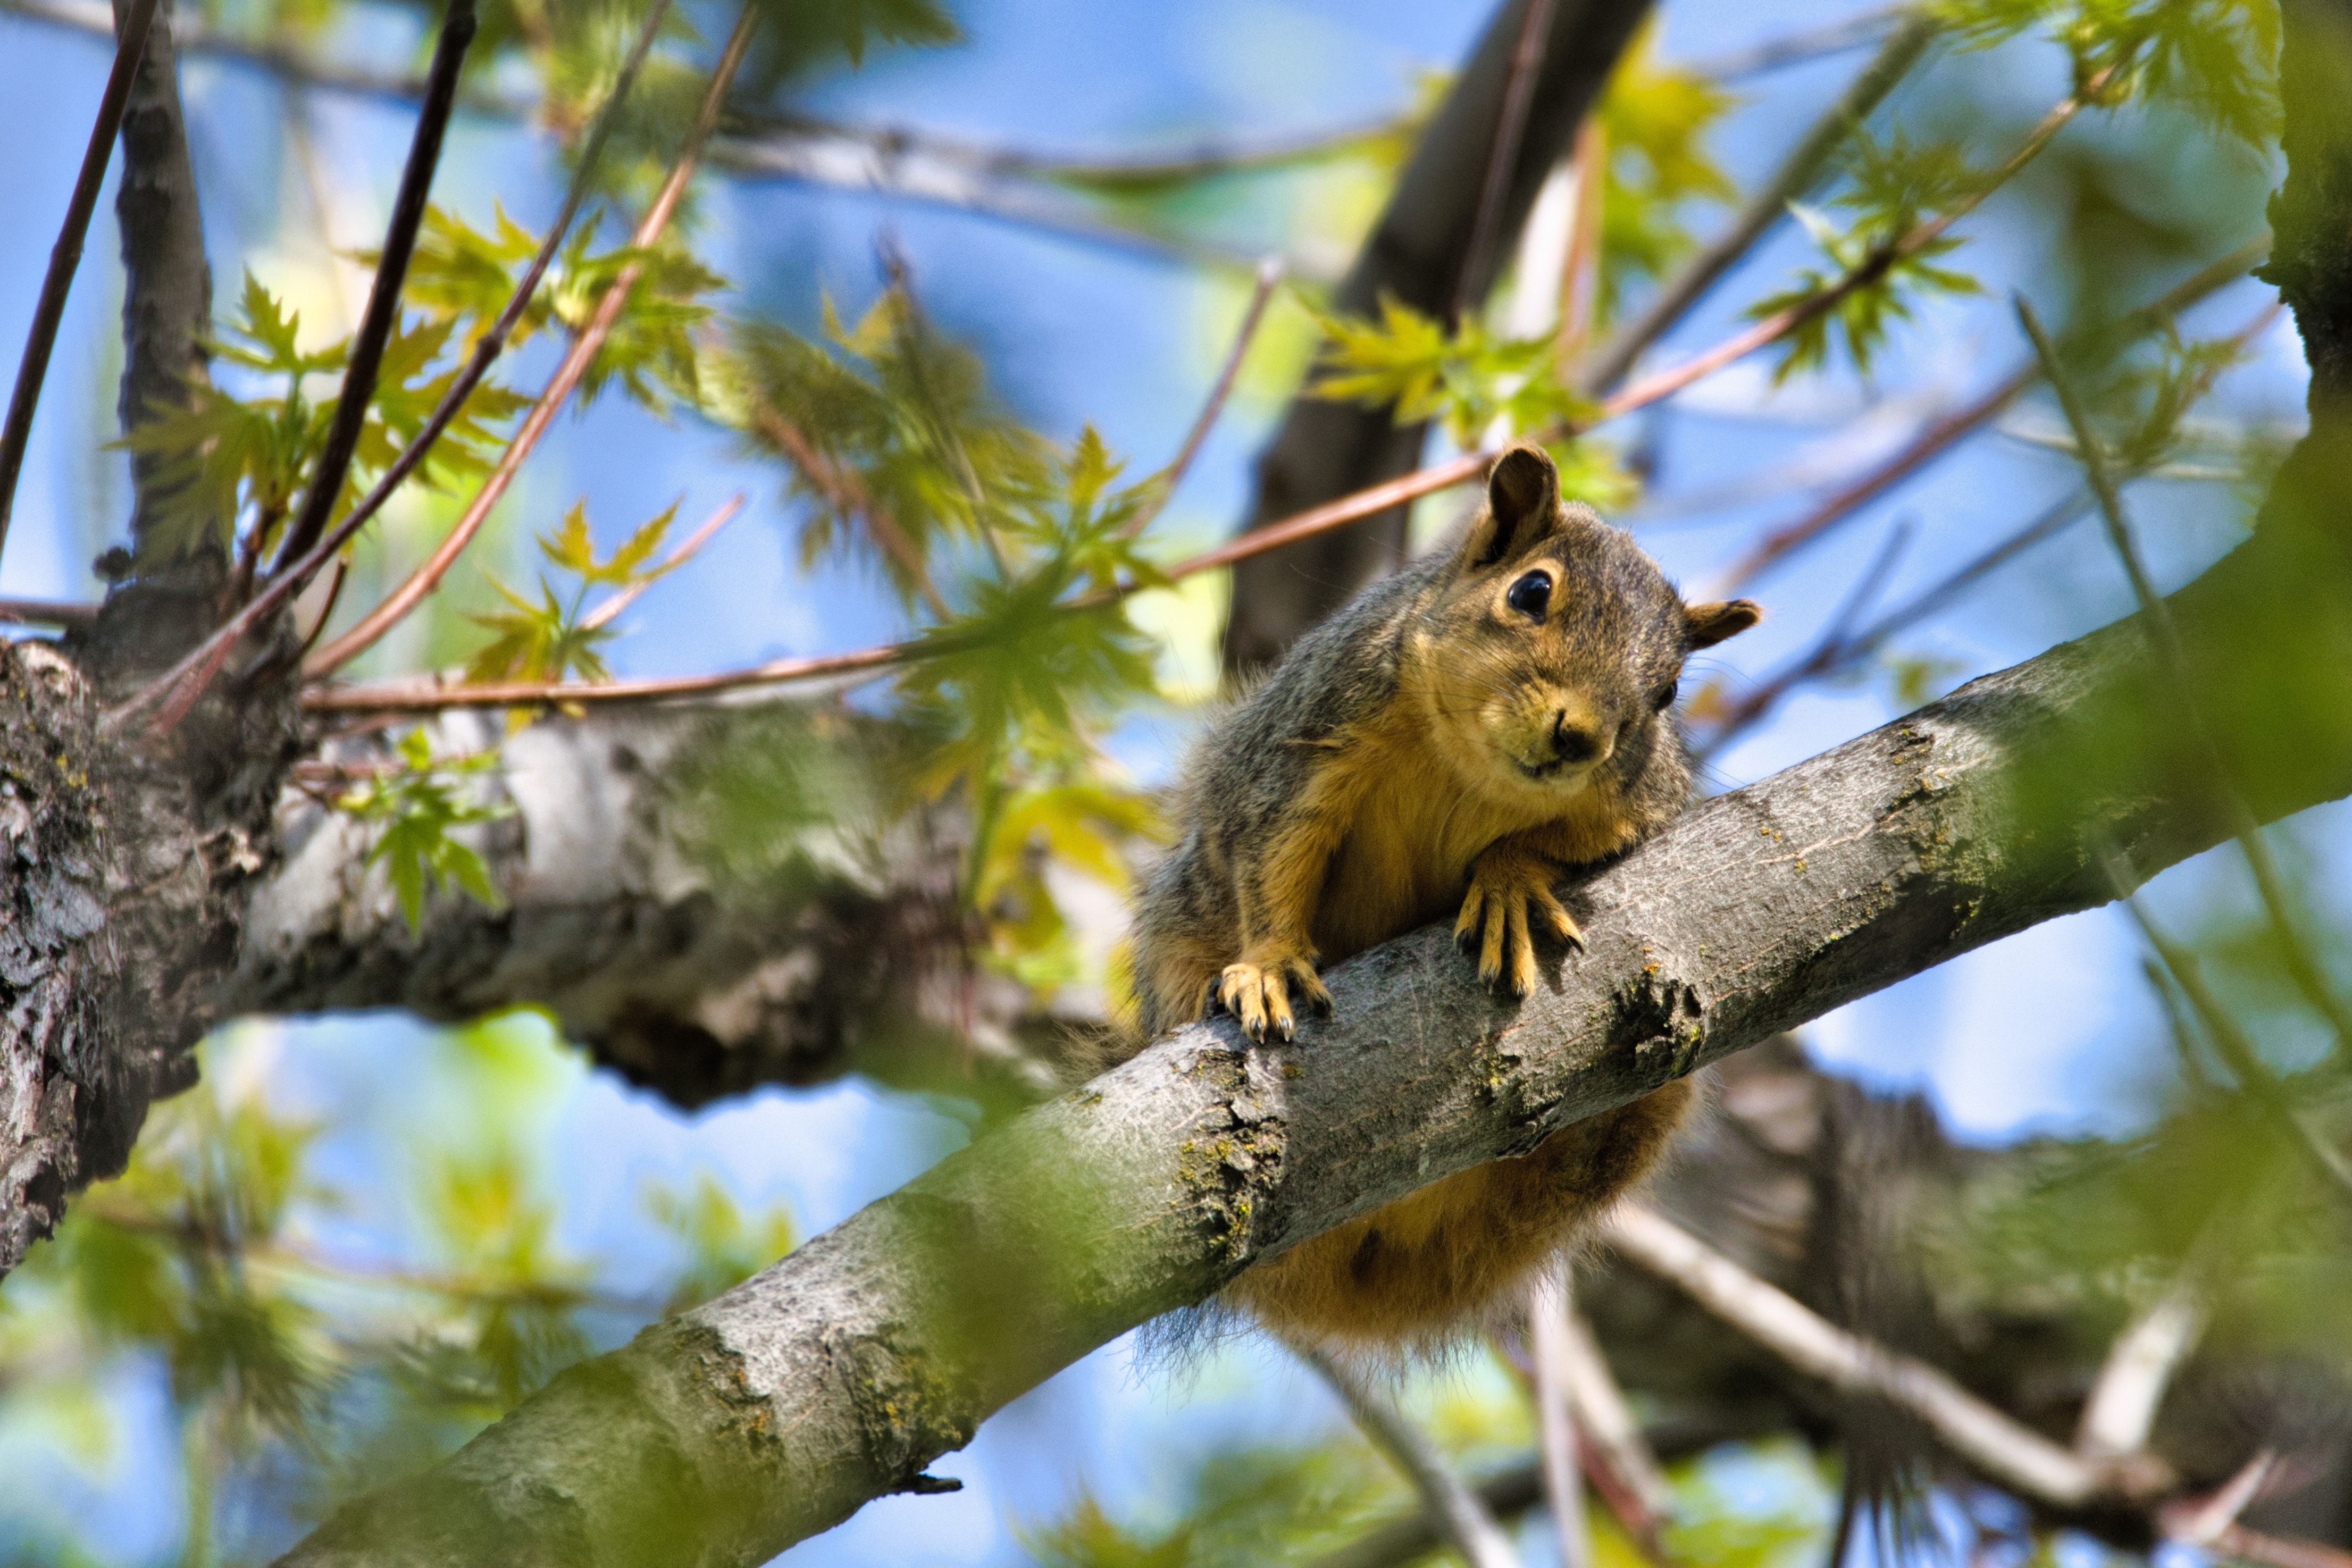
\includegraphics[width=8cm]{demo.jpg}
\centering
  \caption{A very good friend, with good news.}
    \label{fig:demo}
\end{figure}
he other side, if you are only interested on
certain va for documents that include \gls{maths}.lues you can use the contour plot, you 
can use the contour plot, you can use the contour 
plot, you can use the contour plot, you can use 
the contour plot, you \acrshort{vgd} can use the contour plot, 
you can use the contour.  The table \ref{table:1} is an example of referenced \LaTeX elements.
 
\begin{table}[h!]
\centering
\begin{tabular}{||c c c c||} 
 \hline
 Col1 & Col2 & Col2 & Col3 \\ [0.5ex] 
 \hline\hline
 1 & 6 & 87837 & 787 \\ 
 2 & 7 & 78 & 5415 \\
 3 & 545 & 778 & 7507 \\
 4 & 545 & 18744 & 7560 \\
 5 & 88 & 788 & 6344 \\ [1ex] 
 \hline
\end{tabular}
\caption{Table to demonstrate captions and labels}
\label{table:1}
\end{table}

%% Just to fill out the table of contents
\chapter{Case Study 3: Brilliant!}
\section{Section1}
\section{Section2}
\chapter{Discussion - Very Important Thoughts}
\section{A review of things written}
\section{Exciting connections}
\section{Very good analysis}
\chapter{Conclusion - There's more!}
\section{More summaries}
\section{Review of main contributions}
\section{Calls for further research}

% SEE - printing them here, the glossaries work. 
% TODO - why don't they work from within?
\printglossaries


%-----------------------back matter
{\singlespace
% Making the references a "part" rather than a chapter gets it indented at
% level -1 according to the chart: top of page 4 of the document at
% ftp://tug.ctan.org/pub/tex-archive/macros/latex/contrib/tocloft/tocloft.pdf
\addcontentsline{toc}{part}{REFERENCES}
% here for the bibliography, the exported thing needs to be in BetterBibTEX (not latex, I think?) I just know that it's sensitive. 

\bibliographystyle{asudis}
\bibliography{dis}}

\printglossaries
\printglossary[type=\acronymtype]

\renewcommand{\chaptername}{APPENDIX}
\addtocontents{toc}{APPENDIX \par}
\appendix
% This is an appendix chapter because it's included in the back matter.
\chapter{Appendix: More Data!}

\addcontentsline{toc}{part}{BIOGRAPHICAL SKETCH}
\biographicalpage{\\Enter content here.}
\include{vita}
\end{document}